\chapter{Exercices}

\minitoc



\section{Exercices~: spécifier le problème}

Pour ces premiers exercices, nous vous demandons d’imiter la démarche décrite
dans le chapitre \ref{refpblm}, à savoir~:

\begin{itemize}
	\item déterminer quelles sont les données~;
		leur donner un nom et un type~;
	\item déterminer quel est le type du résultat~;
	\item déterminer un nom pertinent pour l’algorithme~;
	\item fournir un résumé graphique~;
	\item donner des exemples.
\end{itemize}

\begin{Exercice}{Somme de 2 nombres}
	Calculer la somme de deux nombres donnés.
	\paragraph{Solution.}%
	\footnote{%
		Nous allons de temps en temps 
		fournir des solutions.
		En algorithmique,
		il y a souvent \textbf{plusieurs} solutions possibles.
		Ce n’est donc pas parce que vous avez trouvé une autre façon de faire qu'elle est fausse.
		Mais il peut y avoir des solutions \textbf{meilleures}
		que d’autres; 
		n’hésitez jamais à montrer la vôtre
		à votre professeur pour avoir son avis.
	}
	Il y a ici clairement 2 données.
	Comme elles n’ont pas de rôle précis,
	on peut les appeler simplement \pc{nombre1}
	et \pc{nombre2}
	(\pc{nb1} et \pc{nb2} sont aussi de bons choix).
	L’énoncé ne dit pas si les nombres sont entiers ou pas;
	restons le plus général possible en prenant des réels.
	Le résultat sera de même type que les données.
	Le nom de l’algorithme pourrait être simplement \pc{somme}.
	Ce qui donne~:
	\begin{center}
		\flowalgodd{nombre1 (réel)}{nombre2 (réel)}{somme}{réel}
	\end{center}			 
	Et voici quelques exemples numériques~:	
	\pc{somme(3, 2)} donne $5$      \quad
	\pc{somme(-3, 2)} donne $-1$    \quad
	\pc{somme(3, 2.5)} donne $5.5$  \quad
	\pc{somme(-2.5, 2.5)} donne $0$.
\end{Exercice}

\begin{Exercice}{Moyenne de 2 nombres}
	Calculer la moyenne de deux nombres donnés.
\end{Exercice}

\begin{Exercice}{Surface d’un triangle}
	Calculer la surface d’un triangle connaissant sa base et sa hauteur.
\end{Exercice}

\begin{Exercice}{Périmètre d’un cercle}
	Calculer le périmètre d’un cercle dont on donne le rayon. 
\end{Exercice}

\begin{Exercice}{Surface d’un cercle}
	Calculer la surface d’un cercle dont on donne le rayon. 
\end{Exercice}

\begin{Exercice}{TVA}
	Si on donne un prix hors TVA, il faut lui ajouter 21\% 
	pour obtenir le prix TTC. Écrire un algorithme qui permet 
	de passer du prix HTVA au prix TTC.
\end{Exercice}

\begin{Exercice}{Les intérêts}
	Calculer les intérêts reçus après 1 an pour un montant placé en 
	banque à du 2\% d’intérêt.
\end{Exercice}

\begin{Exercice}{Placement}
	Étant donné le montant d’un capital placé (en \texteuro) 
	et le taux d’intérêt annuel (en \%), 
	calculer la nouvelle valeur de ce capital après un an.
\end{Exercice}

\begin{Exercice}{Prix TTC}
	Étant donné le prix unitaire d’un produit
	(hors TVA), le taux de TVA (en \%) et la quantité de produit vendue à
	un client, calculer le prix total à payer par ce client.
\end{Exercice}

\begin{Exercice}{Durée de trajet}
	Étant donné la vitesse moyenne en \textbf{m/s}
	d’un véhicule et la distance parcourue en \textbf{km} par ce véhicule,
	calculer la durée en secondes du trajet de ce véhicule.
\end{Exercice}

\begin{Exercice}{Allure et vitesse}
	L’allure d’un coureur est le temps qu’il met pour parcourir 1~km
	(par exemple, $4'37''$).
	On voudrait calculer sa vitesse (en km/h) à partir de son allure.
	Par exemple, la vitesse d’un coureur ayant une allure de
	$4'37''$ est de $13$~km/h. 
\end{Exercice}

\begin{Exercice}{Somme des chiffres}
	Calculer la somme des chiffres
	d’un nombre entier de 3 chiffres.
\end{Exercice}

\begin{Exercice}{Conversion HMS en secondes}
	Étant donné un moment dans la journée donné
	par trois nombres, à savoir, heure, minute et seconde, calculer le
	nombre de secondes écoulées depuis minuit.
\end{Exercice}

\begin{Exercice}{Conversion secondes en heures}
	Étant donné un temps écoulé depuis minuit.
	Si on devait exprimer ce temps sous la forme
	habituelle (heure, minute et seconde),
	que vaudrait la partie "heure".

	Ex~:~10000 secondes donnera 2 heures.
\end{Exercice}

\begin{Exercice}{Conversion secondes en minutes}
	Étant donné un temps écoulé depuis minuit.
	Si on devait exprimer ce temps sous la forme
	habituelle (heure, minute et seconde),
	que vaudrait la partie "minute".

	Ex~:~10000 secondes donnera 46 minutes.
\end{Exercice}

\begin{Exercice}{Conversion secondes en secondes}
	Étant donné un temps écoulé depuis minuit.
	Si on devait exprimer ce temps sous la forme
	habituelle (heure, minute et seconde),
	que vaudrait la partie "seconde".

	Ex~:~10000 secondes donnera 40 secondes.
\end{Exercice}	

\begin{Exercice}{Cote moyenne}
	Étant donné les résultats (cote entière sur
	20) de trois examens passés par un étudiant (exprimés par six nombres,
	à savoir, la cote et la pondération de chaque examen), calculer 
	la moyenne globale exprimée en pourcentage.
\end{Exercice}



\section{Exercices~: premiers algorithmes et programmes}
\label{prem-ex-simple}

Dans ces exercices, nous vous proposons d'écrire un algorithme et de le traduire
en un programme Java. 

\begin{Exercice}{Moyenne de 2 nombres}	
	Calculer la moyenne de deux nombres donnés.
\end{Exercice}

\begin{Exercice}{Surface d’un triangle}
	Calculer la surface d’un triangle 
	connaissant sa base et sa hauteur.
\end{Exercice}

\begin{Exercice}{Périmètre d’un cercle}
	Calculer le périmètre d’un cercle dont on donne le rayon. 
\end{Exercice}

\begin{Exercice}{Surface d’un cercle}
	Calculer la surface d’un cercle dont on donne le rayon. 
\end{Exercice}

\begin{Exercice}{TVA}
	Si on donne un prix hors TVA, il faut lui ajouter 21\% 
	pour obtenir le prix TTC. Écrire un algorithme qui permet 
	de passer du prix HTVA au prix TTC.
\end{Exercice}

\begin{Exercice}{Les intérêts}	
	Calculer les intérêts reçus après 1 an 
	pour un montant placé en banque à du 2\% d’intérêt.
\end{Exercice}

\begin{Exercice}{Placement}
	Étant donné le montant d’un capital placé (en \texteuro) 
	et le taux d’intérêt annuel (en \%), calculer la
	nouvelle valeur de ce capital après un an.
\end{Exercice}

\begin{Exercice}{Conversion HMS en secondes}
	Étant donné un moment dans la journée donné
	par trois nombres, à savoir, heure, minute et seconde, calculer le
	nombre de secondes écoulées depuis minuit.
\end{Exercice}

\begin{Exercice}{Prix TTC}
	Étant donné le prix unitaire d’un produit
	(hors TVA), le taux de TVA (en \%) 
	et la quantité de produit vendue à un client, 
	calculer le prix total à payer par ce client.
\end{Exercice}



\section{Exercices~: tracer un algorithme}

Nous vous proposons de tracer vos algorithmes comme présenté dans le chapitre 
\ref{premalgo} dans la section \ref{tracer}, page \pageref{tracer}.


\begin{Exercice}{Tracer des bouts de code}
	Suivez l’évolution des variables pour les bouts
	d’algorithmes donnés.

	\begin{minipage}{4cm}
		\begin{pseudocode}[1]
			\Decl{a, b, c}{entiers}
			\Let a \Gets 42
			\Let b \Gets 24
			\Let c \Gets a + b
			\Let c \Gets c - 1
			\Let a \Gets 2 * b
			\Let c \Gets c + 1
		\end{pseudocode}
	\end{minipage}
	\quad%
	\begin{minipage}{7cm}
		\begin{tabular}{|>{\centering\arraybackslash}m{1cm}|*{3}{>{\centering\arraybackslash}m{2cm}}|}
			\hline
			\verb_#_ & {a} & {b} & {c}\\
			\hline
			1 & {} & {} & {} \\
			2 & {} & {} & {} \\
			3 & {} & {} & {} \\
			4 & {} & {} & {} \\
			5 & {} & {} & {} \\
			6 & {} & {} & {} \\
			7 & {} & {} & {} \\
			\hline
		\end{tabular}
	\end{minipage}

	\bigskip
	\begin{minipage}{4cm}
		\begin{pseudocode}[1]
			\Decl{a, b, c}{entiers}
			\Let a \Gets 2
			\Let b \Gets a$^3$
			\Let c \Gets b - a$^2$
			\Let a \Gets $\sqrt{c}$
			\Let a \Gets a / a
		\end{pseudocode}
	\end{minipage}
	\quad%
	\begin{minipage}{7cm}
		\begin{tabular}{|>{\centering\arraybackslash}m{1cm}|*{3}{>{\centering\arraybackslash}m{2cm}}|}
			\hline
			\verb_#_ & {a} & {b} & {c}\\
			\hline
			1 & {} & {} & {} \\
			2 & {} & {} & {} \\
			3 & {} & {} & {} \\
			4 & {} & {} & {} \\
			5 & {} & {} & {} \\
			6 & {} & {} & {} \\
			\hline
		\end{tabular}
	\end{minipage}	
\end{Exercice}

\begin{Exercice}{Calcul de vitesse}

	Soit le problème suivant :
	\og
	Calculer la vitesse (en km/h) d’un véhicule 
	dont on donne la durée du parcours (en secondes) 
	et la distance parcourue (en mètres).
	\fg.

	Voici \textit{une} solution : 
	\begin{pseudocode}[1]
		\Algo{vitesseKMH}{\Par{distanceM, duréeS}{réels}}{réel}
		\Decl{distanceKM, duréeH}{réels}
		\Let distanceKM \Gets 1000 * distanceM
		\Let duréeH \Gets 3600 * duréeS
		\Return $\frac{\textrm{distanceKM}}{\textrm{duréeH}}$
	\EndAlgo
\end{pseudocode}

L’algorithme, s’il est correct, devrait donner
une vitesse de 1~km/h pour une distance de 1000~mètres
et une durée de 3600~secondes.
Testez cet algorithme avec cet exemple.

\begin{center}
	\begin{tabular}{|>{\centering\arraybackslash}m{1cm}|*{5}{>{\centering\arraybackslash}m{2cm}}|}
		\hline
		\verb_#_  &  &  & & &  \\			
		\hline
		1 & & & & & \\
		2 & & & & & \\
		3 & & & & & \\
		4 & & & & & \\
		5 & & & & & \\
		\hline
	\end{tabular}
\end{center}

Si vous trouvez qu’il n’est pas correct,
voyez ce qu’il faudrait changer pour le corriger.
\end{Exercice}

\begin{Exercice}{Allure et vitesse}

	L’allure d’un coureur est le temps qu’il met pour parcourir 1~km (par exemple,
	$4'37''$).  On voudrait calculer sa vitesse (en km/h) à partir de son allure.
	Par exemple, la vitesse d’un coureur ayant une allure de $4'37''$ est de
	$12,996389892$~km/h. 

\end{Exercice}

\begin{Exercice}{Cote moyenne}

	Étant donné les résultats (cote entière sur
	20) de trois examens passés par un étudiant (exprimés par six nombres, à savoir,
	la cote et la pondération de chaque examen), calculer la moyenne globale
	exprimée en pourcentage.  

\end{Exercice}





\section{Exercices~: division entière, quotient et reste}

\begin{Exercice}{Calculs}

	Voici quelques petits calculs à compléter faisant intervenir la division entière
	et le reste.  Par exemple~: "14 DIV 3 = 4 reste 2" signifie que 14 DIV 3 = 4 et
	14 MOD 3 = 2.

	\begin{multicols}{2}
		\begin{itemize}
			\item 11 DIV 3 = \_\_\ reste\ \_\_
			\item 3 DIV 11 = \_\_\ reste\ \_\_
			\item 11 DIV \_\_ = 2\ reste\ 3
			\item \_\_ DIV 3 = 3\ reste\ 1
		\end{itemize}
	\end{multicols}
\end{Exercice}

\begin{Exercice}{Les prix ronds}
	Voici un algorithme qui reçoit une somme d’argent exprimée en centimes
	et qui calcule le nombre (entier) de centimes qu’il
	faudrait ajouter à la somme pour tomber sur un prix rond en euros.
	Testez-le avec des valeurs numériques. Est-il correct~?

	\begin{pseudocode}
		\Algo{versPrixRond}{\Par{prixCentimes}{entier}}{entier}
		\Return 100 - (prixCentimes MOD 100)
	\EndAlgo
\end{pseudocode}

\begin{center}
	\begin{tabular}{|c|c|c|c|c|}
		\hline
		test \no & prixCentimes & réponse correcte & valeur retournée & Correct~? \\\hline
		\hline 
		1 & 130 & 70 &  & \\\hline
		2 & 40  & 60 &  & \\\hline
		3 & 99  & 1  &  & \\\hline
		4 & 100 & 0  &  & \\\hline
	\end{tabular}
\end{center}

\end{Exercice}

\bigskip
\begin{Emphase}
	
	\paragraph{Remarque}
	Les exercices qui suivent n’ont pas tous été déjà analysés et ils demandent
	des calculs faisant intervenir des divisions entières, des restes et/ou des
	expressions booléennes.  Comme d’habitude, écrivez la spécification si ça
	n’a pas encore été fait, donnez des exemples, rédigez un algorithme et
	vérifiez-le.

\end{Emphase}

		\begin{Exercice}{Nombre multiple de 5}

			\label{algo:mult5}
			Calculer si un nombre entier donné est un multiple de 5.
			\paragraph{Solution.}
			Dans ce problème,
			il y a une donnée, le nombre à tester.
			La réponse est un booléen
			qui est à vrai si le nombre donné est un multiple de 5.
			\begin{center}
				\flowalgod{nombre (entier)}{multiple5}{booléen}
			\end{center}
			\textbf{Exemples.}
			\begin{multicols}{4}
				\begin{itemize}
					\item \pc{multiple5(4)} donne faux
					\item \pc{multiple5(15)} donne vrai
					\item \pc{multiple5(0)} donne vrai
					\item \pc{multiple5(-10)} donne vrai
				\end{itemize}
			\end{multicols}
			La technique pour vérifier si un nombre est
			un multiple de 5 est de vérifier que le reste
			de la division par 5 donne 0.
			Ce qui donne~:
			\begin{pseudocode}[1]
				\Algo{multiple5}{\Par{nombre}{entier}}{booléen}
				\Return nombre MOD 5 == 0
			\EndAlgo
		\end{pseudocode}
		Vérifions sur nos exemples~:
		\begin{center}
			\begin{tabular}{|c|c|c|c|c|}
				\hline
				test \no & nombre & réponse correcte & valeur retournée & Correct~? \\\hline
				\hline 
				1 & 4   & faux & faux & {\color{ForestGreen}$\checkmark$} \\\hline
				2 & 15  & vrai & vrai & {\color{ForestGreen}$\checkmark$} \\\hline
				3 & 0   & vrai & vrai & {\color{ForestGreen}$\checkmark$} \\\hline
				4 & -10 & vrai & vrai & {\color{ForestGreen}$\checkmark$} \\\hline
			\end{tabular}
		\end{center}
	\end{Exercice}

	\begin{Exercice}{Nombre entier positif se terminant par un 0}
		Calculer si un nombre donné se termine par un 0.
	\end{Exercice}

	\begin{Exercice}{Les centaines}
		Calculer la partie \emph{centaine}
		d’un nombre entier positif quelconque.
	\end{Exercice}

	\begin{Exercice}{Somme des chiffres}
		Calculer la somme des chiffres
		d’un nombre entier positif inférieur à 1000.
	\end{Exercice}

	\begin{Exercice}{Conversion secondes en heures}
		Étant donné un temps écoulé depuis minuit.
		Si on devait exprimer ce temps sous la forme
		habituelle (heure, minute et seconde),
		que vaudrait la partie "heure".

		Ex~:~10000 secondes donnera 2 heures.

		Aide~: L’heure n’est qu’un nombre exprimé en base 60~!
	\end{Exercice}

	\begin{Exercice}{Conversion secondes en minutes}
		Étant donné un temps écoulé depuis minuit.
		Si on devait exprimer ce temps sous la forme
		habituelle (heure, minute et seconde),
		que vaudrait la partie "minute".

		Ex~:~10000 secondes donnera 46 minutes.
	\end{Exercice}

	\begin{Exercice}{Conversion secondes en secondes}
		Étant donné un temps écoulé depuis minuit.
		Si on devait exprimer ce temps sous la forme
		habituelle (heure, minute et seconde),
		que vaudrait la partie "seconde".

		Ex~:~10000 secondes donnera 40 secondes.
	\end{Exercice}	

	\begin{Exercice}{Un double aux dés}

		Écrire un algorithme qui simule le lancer de deux dés
		et indique s’il y a eu un double 
		(les deux dés montrant une face identique).
	\end{Exercice}

	\begin{Exercice}{Année bissextile}

		\label{ex:bissextile}
		Écrire un algorithme qui vérifie si une année est bissextile.

		Pour rappel, les années bissextiles sont les années multiples de 4. 
		Font exception, les multiples de 100 
		(sauf les multiples de 400 qui sont bien bissextiles). 
		Ainsi $2012$ et $2400$ sont bissextiles mais pas $2010$ ni $2100$.
	\end{Exercice}



	\begin{Exercice}{Conversion en heures-minutes-secondes}

		Écrire un algorithme qui permet à l’utilisateur
		de donner le nombre de secondes écoulées depuis minuit
		et qui affiche le moment de la journée correspopcnt
		en heures-minutes-secondes.
		Par exemple, si on est 3726 secondes après minuit
		alors il est 1h2'6''.
	\end{Exercice}




\section{Exercices~: structures alternatives (choix)}			


\begin{Exercice}{Compréhension}
		Tracez cet algorithme avec les valeurs fournies et donnez la valeur de retour.
		\begin{pseudocode}
			\Algo{exerciceA}{a, b~: entiers}{entier}
			\Decl{c}{entier}
			\Let c \Gets 2 * a
			\If{c > b}
			\Let c \Gets c - b
		\EndIf
		\Return c
	\EndAlgo
\end{pseudocode}		
\begin{multicols}{2}
	\begin{itemize}
		\item \pc{exerciceA(2, 5)} = \_\_\_
		\item \pc{exerciceA(4, 1)} = \_\_\_
	\end{itemize}
\end{multicols}	
	\end{Exercice}

	\begin{Exercice}{Simplification d’algorithmes}
		Voici quelques extraits d’algorithmes corrects 
		du point de vue de la syntaxe 
		mais contenant des lourdeurs d’écriture.
		Simplifiez-les.

		\begin{pseudocode}
			\If{ok = vrai}
			\Write nombre
		\EndIf
	\end{pseudocode}

	\begin{pseudocode}
		\If{ok = faux}
		\Write nombre
	\EndIf
\end{pseudocode}

\begin{pseudocode}
	\If{ok = vrai OU ok = faux}
	\Write nombre
\EndIf
		\end{pseudocode}

		\begin{pseudocode}
			\If{ok = vrai ET ok = faux}
			\Write nombre
		\EndIf
	\end{pseudocode}
\end{Exercice}

\begin{Exercice}{Compréhension}
	Tracez ces algorithmes avec les valeurs fournies et donnez la valeur de retour.

	\begin{pseudocode}
		\Algo{exerciceB}{b, a : entiers}{entier}
		\Decl{c}{entier}
		\If{a > b}
		\Let c \Gets a DIV b
		\Else
		\Let c \Gets b MOD a	
	\EndIf
	\Return c
\EndAlgo
		\end{pseudocode}

		\begin{multicols}{2}
			\begin{itemize}
				\item \pc{exerciceB(2, 3)} = \_\_\_
				\item \pc{exerciceB(4, 1)} = \_\_\_
			\end{itemize}
		\end{multicols}

		\begin{pseudocode}
			\Algo{exerciceC}{x1, x2~: entiers}{entier}
			\Decl{ok}{booléen}
			\Let ok \Gets x1 > x2
			\If{ok}
			\Let ok \Gets ok ET x1 = 4
			\Else
			\Let ok \Gets ok OU x2 = 3
		\EndIf
		\If{ok}
		\Let x1 \Gets x1 * 1000
	\EndIf
	\Return x1 + x2
\EndAlgo
		\end{pseudocode}

		\medskip
		\begin{multicols}{2}
			\begin{itemize}
				\item \pc{exerciceC(2, 3)} = \_\_\_
				\item \pc{exerciceC(4, 1)} = \_\_\_	
			\end{itemize}
		\end{multicols}	

	\end{Exercice}	

	\begin{Exercice}{Simplification d’algorithmes}
		Voici quelques extraits d’algorithmes corrects du point de vue de la
		syntaxe mais contenant des lignes inutiles ou des lourdeurs d’écriture.
		Remplacer chacune de ces portions d’algorithme par un minimum
		d’instructions qui auront un effet équivalent.

		\begin{minipage}[t]{7cm}
			\begin{pseudocode}
				\If{condition}
				\Let ok \Gets vrai
				\Else
				\Let ok \Gets faux
			\EndIf
		\end{pseudocode}
	\end{minipage}
	\quad
	\begin{minipage}[t]{7cm}		
		\begin{pseudocode}
			\If{a $>$ b}
			\Let ok \Gets faux
			\Else
			\If{a $\leq$ b}
			\Let ok \Gets vrai
		\EndIf
	\EndIf
\end{pseudocode}
		\end{minipage}
	\end{Exercice}

	\begin{Exercice}{Maximum de 2 nombres}

		Écrire un algorithme qui, étant donné deux nombres quelconques,
		recherche et retourne le plus grand des deux. Attention~! On ne veut
		pas savoir si c’est le premier ou le deuxième qui est
		le plus grand mais bien quelle est cette plus grande valeur. Le
		problème est donc bien défini même si les deux nombres sont
		identiques.

		\textbf{Solution.}
		Une solution complète est disponible dans la fiche \vref{fiche:max2nb}.
	\end{Exercice}

	\begin{Exercice}{Calcul de salaire}
		Dans une entreprise, 
		une retenue spéciale de 15\% est pratiquée 
		sur la partie du salaire mensuel qui dépasse 1200~\texteuro. 
		Écrire un algorithme qui calcule le salaire net à partir du salaire brut. 
		En quoi l’utilisation de constantes convient-elle pour améliorer cet algorithme~?
	\end{Exercice}

	\begin{Exercice}{Fonction de Syracuse}

		Écrire un algorithme qui, étant donné un entier $n$ quelconque,
		retourne le résultat de la fonction
		$f(n)=
		\left\{
			\begin{array}{rl}
				n/2 & si \ n \ est\ pair\\
				3n+1 & si \ n \ est \ impair
			\end{array}
			\right.$
		\end{Exercice}

		\begin{Exercice}{Tarif réduit ou pas}
			Dans une salle de cinéma,
			le tarif plein pour une place est de 8\texteuro{}.
			Les personnes ayant droit au tarif réduit payent 7\texteuro{}.
			Écrire un algorithme qui reçoit un booléen
			indiquant si la personne peut bénéficier du tarif réduit
			et qui retourne le prix à payer.
		\end{Exercice}

		\begin{Exercice}{Maximum de 3 nombres}

			Écrire un algorithme qui, étant donné trois nombres quelconques,
			recherche et retourne le plus grand des trois.
		\end{Exercice}

		\begin{Exercice}{Le signe}

			Écrire un algorithme qui \textbf{affiche} un message indiquant
			si un entier est strictement négatif, nul ou strictement
			positif.
		\end{Exercice}

		\begin{Exercice}{Le type de triangle}
			Écrire un algorithme qui indique si un triangle
			dont on donne les longueurs de ces 3 cotés est~:
			équilatéral (tous égaux), isocèle (2 égaux)
			ou quelconque.
		\end{Exercice}

		\begin{Exercice}{Dés identiques}
			Écrire un algorithme qui lance trois dés
			et indique si on a obtenu 3 dés de valeur identique,
			2 ou aucun.
		\end{Exercice}

		\begin{Exercice}{Grade}

			Écrire un algorithme qui retourne le grade d’un étudiant 
			suivant la moyenne qu’il a obtenue.

			Un étudiant ayant obtenu 
			\begin{itemize}
				\item moins de 50\% n’a pas réussi~;
				\item de 50\% inclus à 60\% exclu a réussi~;
				\item de 60\% inclus à 70\% exclu a une satisfaction~;
				\item de 70\% inclus à 80\% exclu a une distinction~;
				\item de 80\% inclus à 90\% exclu a une grande distinction~;
				\item de 90\% inclus à 100\% inclus a la plus grande distinction.
			\end{itemize}
		\end{Exercice}


		\begin{Exercice}{Numéro du jour}

			Écrire un algorithme qui retourne le numéro du jour de la semaine
			reçu en paramètre (1 pour "lundi", 2 pour "mardi"\dots).
		\end{Exercice}

		\begin{Exercice}{Tirer une carte}

			Écrire un algorithme qui affiche l’intitulé d’une carte
			tirée au hasard dans un paquet de 52 cartes.
			Par exemple, "As de cœur", "3 de pique", "Valet de carreau"
			ou encore "Roi de trèfle".

			\textbf{Remarque}. Il est plus facile de déterminer séparément
			chacune des deux caractéristiques de la carte : couleur et valeur.
		\end{Exercice}

		\begin{Exercice}{Nombre de jours dans un mois}
			Écrire un algorithme qui retourne le nombre de jours dans un mois. 
			Le mois est lu sous forme d’un entier (1 pour janvier\dots).
			On considère dans cet exercice que le mois de février
			comprend toujours 28 jours.
		\end{Exercice}

		\begin{Exercice}{Réussir DEV1}

			Pour réussir l’UE (unité d’enseignement) DEV1,
			il faut que la cote attribuée à cette UE 
			soit supérieure ou égale à 50\%.
			Cette cote tient compte de votre examen intégré
			et de vos interrogations.
			Écrire un algorithme 
			qui reçoit la cote finale (sur 100)
			d’un étudiant pour l’UE DEV1
			et qui indique si l’étudiant a réussi cette UE.
		\end{Exercice}	

		\begin{comment}
		\begin{Exercice}{Réussir GEN1}

			\label{algo:réussirGEN1}
			l'UE (Unité d'enseignement) GEN1 est composée de trois AA (activité d’apprentissage) :
			Mathématique, Communication anglophone et Comptabilité%
			\footnote{%
				Sans parler de Méthodologie qui ne donne pas lieu à une évaluation.
			}.
			Pour réussir cette unité d’enseignement,
			il faut que la cote attribuée à chaque AA soit supérieure ou égale à 50\%.
			Si c'est le cas, la cote attribuée à l'UE est une moyenne \textbf{pondérée}
			des trois cotes d'AA 
			(avec la pondération 6 pour Mathématique et 2 pour les autres AA).

			Écrire un algorithme qui reçoit les 3 cotes (sur 20) d’AA d’un étudiant
			pour l’UE GEN1 et qui \textbf{affiche} un message
			indiquant si l’étudiant a réussi ou pas cette UE.
			S’il a réussi, l’algorithme affiche également la cote d'UE (sur 20).
		\end{Exercice}		
		\end{comment}

		\begin{Exercice}{La fourchette}

			Écrire un algorithme qui, étant donné trois nombres, 
			retourne vrai si le premier des trois 
			appartient à l’intervalle donné par le plus petit et le plus grand 
			des deux autres (bornes exclues) et faux sinon. 
			Qu’est-ce qui change si on inclut les bornes~?
		\end{Exercice}

		\begin{Exercice}{Le prix des photocopies}

			Un magasin de photocopies facture 0,10 \texteuro{} 
			les dix premières photocopies, 
			0,09 \texteuro{} les vingt suivantes 
			et 0,08 \texteuro{} au-delà. 
			Écrivez un algorithme 
			qui reçoit le nombre de photocopies effectuées 
			et qui affiche la facture correspopcnte.
		\end{Exercice}

		\begin{Exercice}{Le stationnement alternatif}

			Dans une rue où se pratique le stationnement alternatif, 
			du 1 au 15 du mois, on se gare du côté des maisons ayant un numéro impair, 
			et le reste du mois, on se gare de l’autre côté. 
			Écrire un algorithme qui, sur base de la date du jour et du numéro de maison
			devant laquelle vous vous êtes arrêté, 
			retourne vrai si vous êtes bien stationné et faux sinon.
		\end{Exercice}





\section{Exercices~: modules et méthodes}

		\begin{Exercice}{Tracer des algorithmes}
			Indiquer quels nombres sont successivement affichés 
			lors de l’exécution des algorithmes ex1, ex2, ex3 et ex4.

			\begin{pseudocode}
				\Algo{ex1}{}{}
				\Decl{x, y}{entiers}
				\Stmt addition(3, 4, x)
				\Write x
				\Let x \Gets 3
				\Let y \Gets 5
				\Stmt addition(x, y, y)
				\Write y
			\EndAlgo
			\Empty
			\Algo{addition}{a\In, b\In, c\Out~:~entiers}{}
			\Decl{somme}{entier}
			\Let somme \Gets a + b
			\Let c \Gets somme
		\EndAlgo
	\end{pseudocode}

	\begin{pseudocode}
		\Algo{ex2}{}{}
		\Decl{a, b}{entiers}
		\Stmt addition(3, 4, a) \Comment voir ci-dessus
		\Write a
		\Let a \Gets 3
		\Let b \Gets 5
		\Stmt soustraction(b, a, b)
		\Write b
	\EndAlgo
	\Empty
	\Algo{soustraction}{a\In, b\In, c\Out~:~entiers}{}
	\Let c \Gets a - b
\EndAlgo
		\end{pseudocode}

		\begin{pseudocode}
			\Algo{ex3}{}{}
			\Decl{a, b, c}{entiers}
			\Stmt calcul(3, 4, c)
			\Write c
			\Let a \Gets 3
			\Let b \Gets 4
			\Let c \Gets 5
			\Stmt calcul(b, c, a)
			\Write a, b, c
		\EndAlgo
		\Empty
		\Algo{calcul}{a\In, b\In, c\Out~:~entiers}{}
		\Let a \Gets 2 * a
		\Let b \Gets 3 * b
		\Let c \Gets a + b
	\EndAlgo
\end{pseudocode}

\begin{pseudocode}
	\Algo{ex4}{}{}
	\Decl{a, b, c}{entiers}
	\Let a \Gets 3
	\Let b \Gets 4
	\Let c \Gets f(b)
	\Write c
	\Stmt calcul2(a, b, c)
	\Write a, b, c
\EndAlgo
\Empty
\Algo{calcul2}{a\In, b\In, c\Out~:~entiers}{}
\Let a \Gets f(a)
\Let c \Gets 3 * b
\Let c \Gets a + c
		\EndAlgo
		\Empty
		\Algo{f}{a\In~:~entier}{entier}
		\Decl{b}{entier}
		\Let b \Gets 2 * a + 1
		\Return b
	\EndAlgo
\end{pseudocode}	
	\end{Exercice}

	\begin{Exercice}{Appels de module}
		Parmi les instructions suivantes (où les variables
		\pc{a}, \pc{b} et \pc{c}
		sont des entiers), lesquelles font correctement appel 
		à l’algorithme d’en-tête suivant~?

		\begin{pseudocode}
			\Entete{PGCD}{a\In,b\In~:~entiers}{entier}
		\end{pseudocode}

		\begin{pseudocode}
			\Stmt [1] a \Gets PGCD(24, 32)
			\Stmt [2] a \Gets PGCD(a, 24)
			\Stmt [3] b \Gets 3 * PGCD(a + b, 2*c) + 120
			\Stmt [4] PGCD(20, 30)
			\Stmt [5] a \Gets PGCD(a, b, c)
			\Stmt [6] a \Gets PGCD(a, b) + PGCD(a, c)
			\Stmt [7] a \Gets PGCD(a, PGCD(a, b))
			\Stmt [8] \Read PGCD(a, b)
			\Stmt [9] \Write PGCD(a, b)
			\Stmt [10] PGCD(a, b) \Gets c
		\end{pseudocode}
	\end{Exercice}

	\begin{Exercice}{Maximum de 4 nombres}
		Écrivez un algorithme qui calcule le maximum de 4 nombres.
	\end{Exercice}

	\begin{Exercice}{Écart entre 2 durées}
		Étant donné deux durées données chacune par trois
		nombres (heure, minute, seconde),
		écrire un algorithme qui calcule
		le délai écoulé entre ces deux durées en heure(s), minute(s),
		seconde(s) sachant que la deuxième durée donnée 
		est plus petite que la première.
	\end{Exercice}

	\begin{comment}
	\begin{Exercice}{Réussir GEN1}
		Reprenons l’exercice \vref{algo:réussirGEN1}.
		Cette fois-ci on ne veut rien afficher
		mais fournir deux résultats~:
		un booléen indiquant si l’étudiant a réussi ou pas
		et un entier indiquant sa cote (qui n’a de sens que s’il a réussi). 
	\end{Exercice}
	\end{comment}

	\begin{Exercice}{Tirer une carte}

		L’exercice suivant a déjà été résolu. 
		Refaites une solution modulaire.

		Écrire un algorithme qui affiche l’intitulé d’une carte
		tirée au hasard dans un paquet de 52 cartes.
		Par exemple, "As de cœur", "3 de pique", "Valet de carreau"
		ou encore "Roi de trèfle".
	\end{Exercice}

	\begin{Exercice}{Nombre de jours dans un mois}
		Écrire un algorithme qui donne le nombre de jours dans un mois.
		Il reçoit en paramètre le numéro du mois (1 pour janvier\dots)
		ainsi que l’année.
		Pour le mois de février, 
		il faudra répondre 28 ou 29 selon que l’année fournie
		est bissextile ou pas.
		Vous devez réutiliser au maximum ce que vous avez déjà fait
		lors d’exercices précédents (cf. exercice \vref{ex:bissextile}).
	\end{Exercice}

	\begin{Exercice}{Valider une date}
		Écrire un algorithme qui valide 
		une date donnée par trois entiers~:~ l’année, le mois et le jour.
		Vous devez réutiliser au maximum ce que vous avez déjà fait
		lors d’exercices précédents.
	\end{Exercice}

	\begin{Exercice}{Généraliser un algorithme}
		Dans l’exercice \vref{algo:mult5},
		nous avons écrit un algorithme 
		pour tester si un nombre est divisible par 5.
		Si on vous demande à présent
		un algorithme pour tester si un nombre est divisible par 3,
		vous le feriez sans peine.
		Idem pour tester la divisibilité par 2, 4, 6, 7, 8, 9\dots{}
		mais vous vous lasseriez bien vite.

		N’est-il pas possible d’écrire un seul algorithme,
		plus général, qui résolve tous ces problèmes d’un coup~?  
	\end{Exercice}





\section{Exercices~: structures itératives}

\subsection{while}

	\begin{Exercice}{Compréhension d’algorithmes}
		Quels sont les affichages réalisés lors de l’exécution
		des algorithmes suivants~?

		\begin{minipage}[t]{.5\linewidth}
			\begin{pseudocode}
				\Algo{boucle1}{}{}
				\Decl{x}{entier}
				\Let x \Gets 0
				\While{x < 12}
				\Let x \Gets x + 2	
			\EndWhile
			\Write x
		\EndAlgo
	\end{pseudocode}
\end{minipage}
\ 
\begin{minipage}[t]{.5\linewidth}
	\begin{pseudocode}
		\Algo{boucle2}{}{}
		\Decl{ok}{booléen}
		\Decl{x}{entier}
		\Let ok \Gets vrai
		\Let x \Gets 5
		\While{ok}
		\Let x \Gets x + 7	
		\Let ok \Gets x MOD 11 $\neq$ 0	
	\EndWhile
	\Write x
\EndAlgo
				\end{pseudocode}
			\end{minipage}
			


				\begin{pseudocode}
					\Algo{boucle3}{}{}
					\Decl{ok}{booléen}
					\Decl{cpt, x}{entiers}
					\Let x \Gets 10
					\Let cpt \Gets 0
					\Let ok \Gets vrai
					\While{ok ET cpt < 3}
					\If{x MOD 2 = 0}
					\Let x \Gets x + 1
					\Let ok \Gets x < 20
					\Else
					\Let x \Gets x + 3
					\Let cpt \Gets cpt + 1
				\EndIf
			\EndWhile
			\Write x
		\EndAlgo
	\end{pseudocode}
		\end{Exercice}

		\begin{Exercice}{Afficher des nombres}

			En utilisant un \pc{\algorithmicwhile},
			écrire un algorithme qui reçoit un entier $n$ positif et affiche
			\begin{enumerate}[label=\alph*)]
				\item les nombres de 1 à $n$~;
				\item les nombres de 1 à $n$ en ordre décroissant~;
				\item les nombres impairs de 1 à $n$~;
				\item les nombres de -n à n~;
				\item les multiples de 5 de 1 à n~;
				\item les multiples de n de 1 à 100.
			\end{enumerate}
		\end{Exercice}




\subsection{for}

		\begin{Exercice}{Compréhension d’algorithmes}
			Quels sont les affichages réalisés lors de l’exécution
			des algorithmes suivants~?

				\begin{pseudocode}
					\Algo{boucle5}{}{}
					\Decl{x}{entier}
					\Decl{ok}{booléen}
					\Let x \Gets 3
					\Let ok \Gets vrai
					\For{i}{1}{5}
					\Let x \Gets x + i
					\Let ok \Gets ok ET (x MOD 2 = 0)
				\EndFor
				\If{ok}
				\Write x
				\Else
				\Write 2 * x
			\EndIf
		\EndAlgo
	\end{pseudocode}
	
	\begin{pseudocode}
		\Algo{boucle6}{}{}
		\Decl{fin}{entiers}
		\For{i}{1}{3}
		\Let fin \Gets 6 * i - 11
		\For[3]{j}{1}{fin}
		\Write 10 * i + j
	\EndFor
\EndFor
				\EndAlgo
			\end{pseudocode}

	\end{Exercice}

	\begin{Exercice}{Afficher des nombres}

		Reprenons un exercice déjà donné avec le \pc{\algorithmicwhile}.
		En utilisant un \pc{\algorithmicfor},
		écrire un algorithme qui reçoit un entier $n$ positif et affiche
		\begin{enumerate}[label=\alph*)]
			\item les nombres de 1 à $n$~;
			\item les nombres de 1 à $n$ en ordre décroissant~;
			\item les nombres de -n à n~;
			\item les multiples de 5 de 1 à n~;
			\item les multiples de n de 1 à 100.
		\end{enumerate}
	\end{Exercice}




\subsection{do while}

	\begin{Exercice}{Compréhension d’algorithmes}
		Quels sont les affichages réalisés lors de l’exécution
		des algorithmes suivants~?

		\begin{pseudocode}
			\Algo{boucle4}{}{}
			\Decl{pair, grand}{booléens}
			\Decl{p, x}{entiers}
			\Let x \Gets 1
			\Let p \Gets 1
			\Repeat
			\Let p \Gets 2 * p
			\Let x \Gets x + p
			\Let pair \Gets x MOD 2 = 0
			\Let grand \Gets x > 15
		\EndRepeat{NON pair ET NON grand}
		\Write x
	\EndAlgo
\end{pseudocode}		

		\end{Exercice}

		\begin{Exercice}{Afficher des nombres}

			Reprenons un exercice déjà fait avec le \pc{\algorithmicwhile}
			et le \pc{\algorithmicfor}
			en utilisant cette fois un \pc{\algorithmicrepeat} \pc{\algorithmicwhile}.
			Écrire un algorithme qui reçoit un entier $n$ positif et affiche
			\begin{enumerate}[label=\alph*)]
				\item les nombres de 1 à $n$~;
				\item les nombres de 1 à $n$ en ordre décroissant~;
				\item les nombres de -n à n~;
				\item les multiples de 5 de 1 à n~;
				\item les multiples de n de 1 à 100.
			\end{enumerate}
		\end{Exercice}


		
\subsection{Exercices récapitulatifs sur les structures répétitives}


		\begin{Exercice}{Afficher les nombres impairs}
			Écrire un algorithme qui demande une série
			de valeurs entières à l’utilisateur
			et qui affiche celles qui sont impaires.
			L’algorithme commence par demander à l’utilisateur
			le nombre de valeurs qu’il désire donner.
		\end{Exercice}

		\begin{Exercice}{Compter les nombres impairs}
			Écrire un algorithme qui demande une série
			de valeurs entières à l’utilisateur
			et qui lui affiche le nombre de valeurs impaires
			qu’il a donné.
			Après chaque valeur entrée,
			l’algorithme demande à l’utilisateur s’il y en a encore d’autres.
		\end{Exercice}

		\begin{Exercice}{Choix de la valeur sentinelle}
			Quelle valeur sentinelle prendrait-on 
			pour additionner une série de cotes d’interrogations~? 
			Une série de températures~?
		\end{Exercice}

		\begin{Exercice}{Afficher les nombres impairs}

			Écrire un algorithme qui demande une série
			de valeurs entières non nulles à l’utilisateur
			et qui affiche celles qui sont impaires.
			La fin des données sera signalée 
			par la valeur sentinelle 0.
		\end{Exercice}

		\begin{Exercice}{Compter le nombre de réussites}

			Écrire un algorithme qui demande une série
			de cotes (entières, sur 20) à l’utilisateur
			et qui affiche le pourcentage de réussites.
			La fin des données sera signalée 
			par une valeur sentinelle que vous pouvez choisir.
		\end{Exercice}

		\begin{Exercice}{Suites}

			Écrire les algorithmes qui affichent
			les $n$ premiers termes des suites suivantes.
			À vous de voir quel est, parmi les 2 modèles 
			décrits dans les exemples précédents, le 
			modèle de solution
			le plus pcpté.
			\begin{enumerate}[label=\alph*)]
				\item -1, -2, -3, -4, -5, -6\dots
				\item 1, 3, 6, 10, 15, 21, 28\dots
				\item 1, 0, 1, 0, 1, 0, 1, 0\dots
				\item 1, 2, 0, 1, 2, 0, 1, 2\dots
				\item 1, 2, 3, 1, 2, 3, 1, 2\dots
				\item 1, 2, 3, 2, 1, 2, 3, 2\dots
			\end{enumerate}			
		\end{Exercice}

\bigskip
\begin{Emphase}

	\paragraph{Remarque}

	Pour les exercices qui suivent, nous vous donnons peu d’indications sur la
	solution à mettre en \oe{}uvre.  À vous de jouer\dots{}

\end{Emphase}
\bigskip

		\begin{Exercice}{Lire un nombre}

			Écrire un algorithme 
			qui demande à l’utilisateur un nombre entre 1 et $n$
			et le retourne.
			Si la valeur donnée n’est pas dans l’intervalle souhaité,
			l’utilisateur est invité à rentrer une nouvelle valeur
			jusqu’à ce qu’elle soit correcte.
			\begin{pseudocode}
				\Entete{lireNb}{\Par{n}{entier}}{entier}
			\end{pseudocode}

			\paragraph{Solution.}
			Si la valeur donnée par l’utilisateur était toujours
			correcte, il suffirait d’écrire~:
			\begin{pseudocode}
				\Algo{lireNb}{\Par{n}{entier}}{entier}
				\Decl{val}{entier}
				\Read{val}
				\Return val
			\EndAlgo
		\end{pseudocode}
		Pour tenir compte des entrées invalides, 
		il faut ajouter une boucle qui
		prévient que la valeur est mauvaise et la redemande.
		Et ceci, tant que c’est incorrect. 
		Ce qui donne~:
		\begin{pseudocode}
			\Algo{lireNb}{\Par{n}{entier}}{entier}
			\Decl{val}{entier}
			\Read{val}
			\While{val<1 OU val>n}
			\Write "valeur incorrecte"
			\Read{val}
		\EndWhile
		\Return val
	\EndAlgo
\end{pseudocode}
La solution qu’on obtient est proche d’une lecture répétée
avec valeur sentinelle.
Dans ce cas, la valeur sentinelle est toute valeur correcte.
	\end{Exercice}

	\begin{Exercice}{Lancé de dés}

		Écrire un algorithme qui lance $n$ fois un dé
		et compte le nombre de fois qu’une certaine valeur est obtenue.
		\begin{pseudocode}
			\Entete{lancerDé}{\Par{n}{entier}, \Par{val}{entier}}{entier}
		\end{pseudocode}
	\end{Exercice}

	\begin{Exercice}{Factorielle}

		Écrire un algorithme qui retourne la factorielle de $n$ (entier positif ou
		nul). Rappel~: la factorielle de $n$, notée $n$!, est le produit des $n$
		premiers entiers strictement positifs. 

		Par convention, 0! = 1.
	\end{Exercice}

	\begin{Exercice}{Produit de 2 nombres}
		Écrire un algorithme qui retourne le produit de deux entiers quelconques
		sans utiliser l’opérateur de multiplication, mais en minimisant le
		nombre d’opérations.
	\end{Exercice}

	\begin{Exercice}{Table de multiplication}

		\begin{minipage}[t]{10cm}
			Écrire un algorithme qui affiche la table de multiplication
			des nombres de 1 à 10
			(cf. l’exemple ci-contre).

			\medskip
			Attention~! Nous somme en algorithmique, 
			ne vous préoccupez pas de la mise en page de ce qui est affiché.
			Ce sera une question importante quand vous traduirez 
			l’algorithme dans un langage de programmation mais pas ici. 
		\end{minipage}
		\qquad
		\begin{minipage}[t]{4cm}
			\begin{verbatim}
			1 x 1 = 1
			1 x 2 = 2
			...
			1 x 10 = 10
			2 x 1 = 2
			...
			10 x 9 = 90
			10 x 10 = 100
			\end{verbatim}
		\end{minipage}		
	\end{Exercice}

	\begin{Exercice}{Double 6}

		Écrire un algorithme qui lance de façon répétée deux dés.
		Il s’arrête lorsqu’il obtient un double 6
		et retourne le nombre de lancés effectués.
	\end{Exercice}

	\begin{Exercice}{Nombre premier}

		Écrire un algorithme qui vérifie si un entier positif est un
		\textbf{nombre premier}. 

		Rappel~:~un nombre est premier s’il n’est divisible que par 1 et par
		lui-même. Le premier nombre premier est 2.
	\end{Exercice}

	\begin{Exercice}{Nombres premiers}

		Écrire un algorithme qui affiche les nombres premiers inférieurs ou
		égaux à un entier positif donné. Le module de cet algorithme fera appel
		de manière répétée mais économique à celui de l’exercice précédent.
	\end{Exercice}

	\begin{Exercice}{Somme de chiffres}

		Écrire un algorithme qui calcule la somme des chiffres qui forment un
		nombre naturel $n$. Attention, on donne au départ \textbf{le} nombre et
		pas ses chiffres. Exemple~: 133045 doit donner comme résultat 16,
		car 1 + 3 + 3 + 0 + 4 + 5 = 16.
	\end{Exercice}

	\begin{Exercice}{Nombre parfait}

		Écrire un algorithme qui vérifie si un entier positif est un
		\textbf{nombre parfait}, c’est-à-dire un nombre égal à la somme de ses
		diviseurs (sauf lui-même). 

		Par exemple, 6 est parfait car 6 = 1 + 2 + 3. 
		De même, 28 est parfait car 28 = 1 + 2 + 4 + 7 + 14.
	\end{Exercice}

	\begin{Exercice}{Décomposition en facteurs premiers}
		Écrire un algorithme qui affiche la décomposition 
		d’un entier en facteurs premiers. 
		Par exemple, $1001880$ donnerait comme décomposition
		$2^3 * 3^2 * 5 * 11^2 * 23$.
	\end{Exercice}

	\begin{Exercice}{Nombre miroir}

		Le miroir d’un nombre est le nombre obtenu
		en lisant les chiffres de droite à gauche.
		Ainsi le nombre miroir de $4209$ est $9024$.
		Écrire un algorithme qui calcule le miroir
		d’un nombre entier positif donné.
	\end{Exercice}

	\begin{Exercice}{Palindrome}

		Écrire un algorithme qui vérifie si un entier donné 
		forme un palindrome ou non. 
		Un nombre palindrome est un nombre qui lu dans un sens 
		(de gauche à droite) est identique au nombre lu dans l’autre sens 
		(de droite à gauche). 
		Par exemple, $1047401$ est un nombre palindrome.
	\end{Exercice}

	\begin{Exercice}{Jeu de la fourchette}

		Écrire un algorithme qui simule le jeu de la
		fourchette. Ce jeu consiste à essayer de découvrir un nombre quelconque
		compris entre 1 et 100 inclus, tiré au sort par l’ordinateur. 
		L’utilisateur a droit à huit essais
		maximum. À chaque essai, l’algorithme devra afficher un message
		indicatif «~nombre donné trop petit~» ou «~nombre donné trop grand~».
		En conclusion, soit «~bravo, vous avez trouvé en [nombre] essai(s)~» soit
		«~désolé, le nombre était [valeur]~».
	\end{Exercice}







\section{Exercices~: tableaux}


	\begin{Exercice}{Déclarer et initialiser}
		Écrire un algorithme qui déclare un tableau de 100 chaines
		et met votre nom dans la 3\ieme{} case du tableau.
	\end{Exercice}

	\begin{Exercice}{Initialiser un tableau à son indice}
		Écrire un algorithme qui déclare un tableau de 100 entiers
		et initialise chaque élément à la valeur de son indice.
		Ainsi, la case numéro $i$ contiendra la valeur $i$.
	\end{Exercice}

	\begin{Exercice}{Initialiser un tableau aux valeurs de 1 à 100}
		Écrire un algorithme qui déclare un tableau de 100 entiers
		et y met les nombres de 1 à 100.
	\end{Exercice}

	\begin{Exercice}{Compréhension}
		Expliquez la différence entre \pc{tab[i] \Gets tab[i+1]}
		et \pc{tab[i] \Gets tab[i]+1}.
	\end{Exercice}



	\begin{Exercice}{Trouver les entêtes}
		Écrire les entêtes (et uniquement les entêtes)
		des algorithmes qui résolvent les problèmes suivants~:
		\begin{enumerate}[label=\alph*)]
			\item
				Écrire un algorithme qui 
				inverse le signe de tous les éléments négatifs dans un tableau d’entiers.
			\item
				Écrire un algorithme qui
				donne le nombre d’éléments négatifs dans un tableau d’entiers.
			\item
				Écrire un algorithme qui
				détermine si un tableau d’entiers contient au moins un nombre négatif.
			\item
				Écrire un algorithme qui
				détermine si un tableau de chaines contient
				une chaine donnée en paramètre.
			\item
				Écrire un algorithme qui
				détermine si un tableau de chaines contient
				au moins deux occurrences de la même chaine,
				quelle qu’elle soit.
			\item
				Écrire un algorithme qui 
				retourne un tableau donnant les $n$ premiers nombres premiers,
				où $n$ est un paramètre de l’algorithme.
			\item
				Écrire un algorithme qui 
				reçoit un tableau d’entiers
				et retourne un tableau de booléens de la même taille
				où la case $i$ indique si oui ou non
				le nombre reçu dans la case $i$ est strictement positif.
		\end{enumerate}
	\end{Exercice}


	\begin{Exercice}{Inverser le signe des éléments}
		Écrire un algorithme qui 
		inverse le signe de tous les éléments négatifs dans un tableau d’entiers.
	\end{Exercice}

	\begin{Exercice}{Somme}

		Écrire un algorithme qui reçoit en paramètre le tableau
		\pc{tabEnt} de $n$ entiers 
		et qui retourne la somme de ses éléments.
	\end{Exercice}

	\begin{Exercice}{Nombre d’éléments d’un tableau}
		Écrire un algorithme qui reçoit en paramètre le tableau
		\pc{tabRéels} de $n$ réels et qui
		retourne le nombre d’éléments du tableau.
	\end{Exercice}

	\begin{Exercice}{Compter les éléments négatifs}
		Écrire un algorithme qui
		donne le nombre d’éléments négatifs dans un tableau d’entiers.
	\end{Exercice}


	\begin{Exercice}{Y a-t-il une copie parfaite~?}

		Écrire un algorithme qui reçoit en paramètre le tableau
		\pc{cotes} de $n$ entiers représentant les cotes des étudiants 
		et qui retourne un booléen 
		indiquant s’il contient \textbf{au moins} une fois la valeur 20. 
	\end{Exercice}

	\begin{Exercice}{Y a-t-il une seule copie parfaite~?}

		Écrire un algorithme qui reçoit en paramètre le tableau
		\pc{cotes} de $n$ entiers représentant les cotes des étudiants 
		et qui retourne un booléen 
		indiquant s’il contient \textbf{exactement} une fois la valeur 20. 
	\end{Exercice}

	\begin{Exercice}{Lancers de deux dés}

		Écrire un algorithme qui lance $n$ fois deux dés
		et compte le nombre de fois que chaque somme apparait.
		\begin{pseudocode}
			\Entete{lancers2Dés}{\Par{n}{entier}}{\Array[2]{12}{entiers}}
		\end{pseudocode}
	\end{Exercice}

	\begin{Exercice}{Nombre de jours dans un mois}

		Écrire un algorithme qui reçoit un numéro de mois (de 1 à 12)
		ainsi qu’une année et donne le nombre de jours dans ce mois
		(en tenant compte des années bissextiles).
		N’hésitez pas à réutiliser des algorithmes déjà écrits.
	\end{Exercice}




	\begin{Exercice}{Éviter la double inscription}
		Comment modifier l’algorithme d’inscription
		pour s’assurer qu’un étudiant ne s’inscrive pas deux fois~?
	\end{Exercice}

	\begin{Exercice}{Limite au nombre d’inscriptions}
		Comment modifier l’algorithme d’inscription
		pour refuser une inscription si le nombre maximal
		de participants est atteint
		en supposant que ce maximum est égal à la taille physique du tableau~?
	\end{Exercice}

	\begin{Exercice}{Vérifier la désinscription}
		Que se passerait-il avec l’algorithme
		de désinscription tel qu’il est
		si on demande à désinscrire un étudiant non inscrit~?
		Que suggérez-vous comme changement~?
	\end{Exercice}


	\begin{Exercice}{Calcul de complexités}
		Quelle est la complexité d’un algorithme qui~:		
		\begin{enumerate}[label=\alph*)]
			\item 
				recherche le maximum d’un tableau de $n$ éléments~?
			\item 
				remplace par 0 toutes les occurrences du maximum 
				d’un tableau de $n$ éléments~?
			\item 
				vérifie si un tableau contient deux éléments égaux~?
				%\item 
				%	trie par recherche des minima successifs~?
			\item 
				vérifie si les éléments d’un tableau forment un palindrome~?
			\item
				cherche un élément dans un tableau 
				en essayant des cases au hasard jusqu’à le trouver~?
		\end{enumerate}
	\end{Exercice}

	\begin{Exercice}{Gestion des données}
		Comparer les algorithmes d’ajout, 
		de recherche et de suppression
		de valeurs dans le cas d’un tableau trié
		et d’un tableau non trié.
	\end{Exercice}

	\begin{Exercice}{Réflexion}
		L’algorithme de recherche dichotomique 
		est-il toujours à préférer à
		l’algorithme de recherche linéaire~?
	\end{Exercice}



	
\bigskip
\begin{Emphase}
	\paragraph{Remarque}
	Voici quelques exercices
	qui reprennent les différentes notions vues sur les tableaux.
	Pour chacun d’entre-eux~:
	\begin{itemize}
	\item
		demandez-vous quel est le problème le plus proche déjà
		rencontré et voyez comment adapter la solution~;
	\item
		indiquez la complexité de votre solution~;
	\item
		décomposez votre solution en plusieurs algorithmes 
		si ça peut améliorer la lisibilité~;
	\item
		testez votre solution dans le cas général
		et dans les éventuels cas particuliers.
	\end{itemize}
\end{Emphase}
\bigskip
	
	\begin{Exercice}{Renverser un tableau}
		
		Écrire un algorithme qui reçoit en paramètre 
		le tableau \pc{tabCar} de $n$ caractères, 
		et qui «~renverse~» ce tableau, 
		c’est-à-dire qui permute le premier élément avec le dernier, 
		le deuxième élément avec l’avant-dernier et ainsi de suite.
	\end{Exercice}
	
	\begin{Exercice}{Tableau symétrique~?}
		Écrire un algorithme qui reçoit en paramètre 
		le tableau \pc{tabChaines} de $n$ chaines 
		et qui vérifie si ce tableau est symétrique, 
		c’est-à-dire si le premier élément est identique au dernier, 
		le deuxième à l’avant-dernier et ainsi de suite.
	\end{Exercice}
		
	\begin{Exercice}{Maximum}
		
		Écrire un algorithme qui reçoit en paramètre le tableau
		\pc{tabEnt} de $n$ entiers et qui
		retourne la plus \textbf{grande} valeur de ce tableau.
	\end{Exercice}
		
	\begin{Exercice}{Minimum}
		
		Écrire un algorithme qui reçoit en paramètre le tableau
		\pc{tabEnt} de $n$ entiers et qui
		retourne la plus \textbf{petite} valeur de ce tableau. Idem pour le minimum.
	\end{Exercice}
	
	\begin{Exercice}{Indice du maximum/minimum}
		\label{ex:indiceminmax}
		
		Écrire un algorithme qui reçoit en paramètre 
		le tableau \pc{tabEnt} de $n$ entiers 
		et qui retourne l’indice de l’élément contenant 
		la plus grande valeur de ce tableau. 
		En cas d’ex-æquo, c’est l’indice le plus petit qui sera renvoyé.
		
		Que faut-il changer pour renvoyer l’indice le plus grand~?
		Et pour retourner l’indice du minimum~? 
		Réécrire l’algorithme de l’exercice précédent en utilisant celui-ci.
	\end{Exercice}
		
	\begin{Exercice}{Tableau ordonné~?}
		
		Écrire un algorithme qui reçoit en paramètre 
		le tableau \pc{valeurs} de $n$ entiers 
		et qui vérifie si ce tableau est ordonné 
		(strictement) croissant sur les valeurs. 
		L’algorithme retournera \pc{vrai} si le tableau est ordonné,
		\pc{faux} sinon.
	\end{Exercice}
	
	\begin{Exercice}{Remplir un tableau}
		On souhaite remplir un tableau de 20 éléments avec
		les entiers de 1 à 5, chaque nombre étant répété quatre fois.
		On voudrait deux variantes :
		\begin{enumerate}[label=\alph*)]
		\item
			D'abord une version
			où les nombres identiques sont groupés :
			d'abord tous les 1 puis tous les 2, \dots
			
			\begin{tabular}{|c|c|c|c|c|c|c|c|c|c|c|c|c|c|}
			\hline
			1 & 1 & 1 & 1 & 2 & 2 & 2 & 2 & 3 & 3 & 3 & 3 & 4 & 4 \\
			\hline
			\end{tabular}
			\begin{flushright}
			\par\hspace{3cm}
			\begin{tabular}{|c|c|c|c|c|c|}
			\hline
			4 & 4 & 5 & 5 & 5 & 5\\
			\hline
			\end{tabular}
			\end{flushright}
		\item
			Ensuite une version où on trouve dans le tableau
			les valeurs 1, 2, 3, 4, 5 qui se suivent, quatre fois.
			
			\begin{tabular}{|c|c|c|c|c|c|c|c|c|c|c|c|c|c|}
			\hline
			1 & 2 & 3 & 4 & 5 & 1 & 2 & 3 & 4 & 5 & 1 & 2 & 3 & 4 \\ 
			\hline
			\end{tabular}
			\begin{flushright}
			\par\hspace{3cm}
			\begin{tabular}{|c|c|c|c|c|c|}
			\hline
			5 & 1 & 2 & 3 & 4 & 5 \\
			\hline
			\end{tabular}
			\end{flushright}
		\end{enumerate}
		\smallskip
		\textbf{Remarque} : 
		Il existe de nombreuses façons de résoudre ce problème.
		On peut par exemple utiliser deux boucles imbriquées.
		On peut aussi adapter un algorithme de génération de suites.
	\end{Exercice}
	
	\begin{Exercice}{Positions du minimum}
		
		Écrire un algorithme qui reçoit en paramètre le tableau
		\pc{cotes} de $n$ entiers et qui
		affiche le ou les indice(s) des éléments 
		contenant la valeur minimale du tableau.
	
		\begin{enumerate}[label=\alph*)]
		\item 
			Écrire une première version «~classique~» avec deux parcours de tableau
		\item
			Écrire une deuxième version qui ne parcourt qu’une seule fois 
			\pc{cotes} en
			stockant dans un deuxième tableau (de quelle taille~?)
			les indices du plus petit élément
			rencontrés (ce tableau étant à chaque fois réinitialisé lorsqu’un
			nouveau minimum est rencontré)
		\item
			Écrire une troisième version qui \textbf{retourne} 
			le tableau contenant les indices.
			Écrire également un algorithme 
			qui appelle cette version puis affiche les indices reçus. 
		\end{enumerate}
	\end{Exercice}
	
	\begin{Exercice}{Occurrence des chiffres}
		
		Écrire un algorithme qui reçoit 
		un nombre entier positif ou nul en paramètre
		et qui retourne un tableau de 10 entiers
		indiquant, pour chacun de ses chiffres, 
		le nombre de fois qu’il apparait dans ce nombre. 
		Ainsi, pour le nombre 10502851125, on retournera
		le tableau \{2,3,2,0,0,3,0,0,1,0\}.
	\end{Exercice}
	
	\begin{Exercice}{Les doublons}
		
		Écrire un algorithme qui vérifie 
		si un tableau de chaines
		contient au moins 2 éléments égaux.
	\end{Exercice}	
	\bigskip
	
	\begin{Exercice}{Le crible d’Ératosthène}
		\begin{quote}
			\og{} Le crible d’Ératosthène est un procédé 
			qui permet de trouver tous les nombres premiers inférieurs 
			à un certain entier naturel donné N.
			L’algorithme procède par élimination~: 
			il s’agit de supprimer d’une table des entiers de 2 à N 
			tous les multiples d’un entier. 
			En supprimant tous les multiples, 
			à la fin il ne restera que les entiers qui ne sont multiples d’aucun entier, 
			et qui sont donc les nombres premiers.
			On commence par rayer les multiples de 2, 
			puis à chaque fois on raye les multiples du plus petit entier restant.
			On peut s’arrêter lorsque le carré du plus petit entier restant 
			est supérieur au plus grand entier restant, car dans ce cas, 
			tous les non-premiers ont déjà été rayés précédemment.\fg{}
			(source~: Wikipédia)
		\end{quote}
		Le tableau dont il est question peut être un simple tableau
		de booléens; le booléen en position "i" indiquant 
		si le nombre "i" est premier ou pas.

		Écrire un algorithme qui reçoit un entier $n$
		et affiche tous les entiers premiers de $1$ à $n$.
	\end{Exercice}
	
	\begin{Exercice}{Mastermind}
		
		Dans le jeu du Mastermind, 
		un joueur A doit trouver une combinaison de $n$ pions de couleur, 
		choisie et tenue secrète par un autre joueur B. 
		Cette combinaison peut contenir éventuellement des pions de même couleur. 
		À chaque proposition du joueur A, 
		le joueur B indique le nombre de pions de la proposition 
		qui sont corrects et bien placés 
		et le nombre de pions corrects mais mal placés. 
		
		Les propositions du joueur A, 
		ainsi que la combinaison secrète du joueur B
		sont contenues dans des tableaux de $n$ composantes de type chaine.
		
		Écrire l’algorithme suivant qui renvoie dans les variables
		\pc{bienPlacés} et \pc{malPlacés}
		respectivement le nombre de pions bien placés et mal placés 
		dans la «~proposition~» du joueur A en la comparant 
		à la «~solution~» cachée du joueur B.
	
		\begin{pseudocode}
		\Entete{testerProposition}{
			\Par{proposition\In, solution\In}{\Array{n}{chaines}}, 
			\\\hfill 
			\Par{bienPlacés\Out, malPlacés\Out}{entiers}}{}
		\end{pseudocode}
	\end{Exercice}
	




	
	
	
	
\section{Exercices~: chaine et String}

	\begin{Exercice}{Calcul de fraction}
		Écrire un algorithme 
		qui reçoit une fraction sous forme de chaine, 
		et retourne la valeur numérique de celle-ci. 
		Par exemple, si la fraction donnée est "5/8", 
		l’algorithme renverra 0,625. 
		On peut considérer que la fraction donnée est correcte, 
		elle est composée de 2 entiers séparés 
		par le caractère de division '/'.

		\paragraph{Solution.}
		Voici une solution possible.
		\begin{pseudocode}
			\Algo{calculerFraction}{\Par{fraction}{string}}{real}
			\Decl{posFraction, numérateur, dénominateur}{integer}
			\Let posFraction \Gets position(fraction,"/")
			\Let numérateur \Gets nombre(souschaine(fraction,1,posFraction-1))
			\Let dénominateur \Gets nombre(souschaine(
				\Let\Indent fraction,
				\Let\Indent posFraction+1,
				\Let\Indent long(fraction)-posFraction))
			\Return numérateur / dénominateur
		\EndAlgo
	\end{pseudocode}
\end{Exercice}

\begin{Exercice}{Conversion de nom}
	Écrire un algorithme 
	qui reçoit le nom complet d’une personne 
	dans une chaine sous la forme "nom, prénom" 
	et la renvoie au format "prénom nom" 
	(sans virgule séparatrice). 
	Exemple~: "De Groote, Jan" deviendra "Jan De Groote".	
\end{Exercice}

\begin{Exercice}{Gauche et droite}
	Écrire un algorithme \pc{gauche} 
	et un \pc{droite}
	qui retourne la chaine formée respectivement 
	des n premiers et des n derniers caractères d’une chaine donnée.	
\end{Exercice}

\begin{Exercice}{Grammaire}
	Écrire un algorithme 
	qui met un mot en « ou » au pluriel. 
	Pour rappel, 
	un mot en « ou » prend un « s » à l’exception des 7 mots 
	bijou, caillou, chou, genou, hibou, joujou et pou qui prennent 
	un « x » au pluriel. 
	Exemple~: un clou, des clous, un hibou, des hiboux. 
	Si le mot soumis à l’algorithme n’est pas un mot en « ou », 
	un message adéquat sera affiché.
\end{Exercice}

\begin{Exercice}{Normaliser une chaine}
	Écrire un module qui reçoit une chaine et retourne une autre chaine,
	version normalisée de la première.
	Par normalisée, on entend~:~enlever tout ce qui n’est pas une lettre 
	et tout mettre en majuscule.
	\\Exemple~:~"Le <COBOL>, c’est la santé~!" devient "LECOBOLCESTLASANTE".
\end{Exercice}

\begin{Exercice}{Les palindromes}
	Cet exercice a déjà été réalisé pour des entiers, 
	en voici 2 versions « chaine »~! 
	\begin{enumerate}[label=\alph*)]
		\item 
			Écrire un algorithme qui vérifie 
			si un mot donné sous forme de chaine 
			constitue un palindrome 
			(comme par exemple "kayak", "radar" ou "saippuakivikauppias" 
			(marchand de savon en finnois)
		\item
			Écrire un algorithme qui vérifie 
			si une phrase donnée sous forme de chaine constitue un palindrome 
			(comme par exemple "Esope reste ici et se repose" 
			ou "Tu l’as trop écrasé, César, ce Port-Salut~!"). 
			Dans cette seconde version, 
			on fait abstraction des majuscules/minuscules 
			et on néglige les espaces et tout signe de ponctuation.
	\end{enumerate}
\end{Exercice}

\begin{Exercice}{Le chiffre de César}
	\label{ex:cesar}
	Depuis l’antiquité, les hommes politiques, les militaires, 
	les hommes d’affaires cherchent à garder secret les messages
	importants qu’ils doivent envoyer.
	L’empereur César utilisait une technique (on dit un \emph{chiffrement})
	qui porte à présent son nom~:
	remplacer chaque lettre du message par la lettre qui se situe 
	$k$ positions plus loin dans l’alphabet (cycliquement).

	Exemple~:~si $k$ vaut $2$, 
	alors le texte clair "CESAR" devient "EGUCT" lorsqu’il est chiffré 
	et le texte "ZUT" devient "BWV".

	Bien sûr, il faut que l’expéditeur du message et le récepteur
	se soient mis d’accord sur la valeur de $k$.

	On vous demande d’écrire un algorithme qui reçoit une chaine ne contenant
	que des lettres majuscules ainsi que la valeur de $k$ et qui retourne
	la version chiffrée du message.

	On vous demande également d’écrire l’algorithme de déchiffrement.
	Cet algorithme reçoit un message chiffré et la valeur de $k$ qui a été
	utilisée pour le chiffrer et retourne le message en clair.
	Attention~! Ce second algorithme est \textbf{très simple}.
\end{Exercice}

\begin{Exercice}{Remplacement de sous-chaines}
	Écrire un algorithme 
	qui remplace dans une chaine donnée 
	toutes les sous-chaines ch1 par la sous-chaine ch2. 
	Attention, 
	cet exercice est plus coriace qu’il n’y parait à première vue\dots~
	Assurez-vous que votre code n’engendre pas de boucle infinie. 
\end{Exercice}	










\section{Exercices~: structures et classes}

Dans ces exercices nous supposons que vous avez au préalable écrit les
structures et classes \pc{Moment}, \pc{Point}… telles que décrites dans le
chapitre \ref{structures-classes} p~\pageref{structures-classes}.

\begin{Exercice}{Conversion moment-secondes}
	Écrire un module qui reçoit en paramètre un
	moment d’une journée et qui retourne le nombre de secondes écoulées
	depuis minuit jusqu’à ce moment.
\end{Exercice}

\begin{Exercice}{Conversion secondes-moment}
	Écrire un module qui reçoit en paramètre un
	nombre de secondes écoulées dans une journée à partir de minuit et qui
	retourne le moment correspondant de la journée.
\end{Exercice}

\begin{Exercice}{Temps écoulé entre 2 moments}
	Écrire un module qui reçoit en paramètres deux
	moments d’une journée et qui retourne le nombre de secondes séparant
	ces deux moments.
\end{Exercice}

\begin{Exercice}{Milieu de 2 points}
	Écrire un module recevant deux points du plan 
	et qui retourne le point situé au milieu des deux.
\end{Exercice}

\begin{Exercice}{Distance entre 2 points}
	Écrire un module recevant les coordonnées de
	deux points distincts du plan et qui retourne
	la distance entre ces deux points.
\end{Exercice}

\begin{Exercice}{Un cercle}
	Définir un type \textbf{Cercle} pouvant décrire de façon
	commode un cercle quelconque dans un espace à deux dimensions. 	
	Écrire ensuite

	\begin{enumerate}[label=\alph*)]
		\item {
			un module calculant la surface du cercle reçu en paramètre~;}
		\item {
				un module recevant 2 points en paramètre et retournant le cercle dont le
			diamètre est le segment reliant ces 2 points~;}
		\item {
			un module qui détermine si un point donné est dans un cercle~;}
		\item {
				un module qui indique si 2 cercles ont une intersection.
			}
	\end{enumerate}
\end{Exercice}


\begin{Exercice}{Un rectangle}

	Définir un type \textbf{Rectangle} pouvant décrire de façon
	commode un rectangle dans un espace à deux dimensions et dont les côtés
	sont parallèles aux axes des coordonnées. 	
	Écrire ensuite

	\begin{enumerate}[label=\alph*)]
		\item {
			un module calculant le périmètre d’un rectangle reçu en paramètre~;}
		\item {
			un module calculant la surface d’un rectangle reçu en paramètre~;}
		\item {
				un module recevant en paramètre un rectangle R et les coordonnées
				d’un point P, et renvoyant 
				\textbf{vrai} si et seulement si le point P est à
			l’intérieur du rectangle R~;}
			%\item {
				%un module recevant en paramètre un rectangle R et les coordonnées
				%d’un point P, et renvoyant 
				%\textbf{vrai} si et seulement si le point P est sur le bord du
				%rectangle R~;}
			%\item {
				%un module recevant en paramètre deux rectangles et renvoyant la valeur
				%booléenne \textbf{vrai} si et seulement si ces deux rectangles ont une
				%intersection.}
	\end{enumerate}
\end{Exercice}

\begin{Exercice}{Validation de date}
	Écrire un algorithme qui valide une date reçue en paramètre 
	sous forme d’une structure.
\end{Exercice}





\section{Exercices récapitulatifs}
\section{Exercices récapitulatifs}

	La plupart des exercices qui suivent sont inspirés d’anciens examens.  Ils
	sont assez conséquents et reprennent la plupart des notions vues dans ce
	cours.

	\begin{Exercice}{AEBBCLRS}

		\begin{quote}
		Le Scrabble est un jeu de lettres, où le but est de former des mots
		ayant le score le plus élevé possible.  Pour calculer le score d’un mot,
		une valeur est associée à chaque lettre de l’alphabet.  Par exemple la
		lettre \texttt{A} vaut 1, \texttt{V} vaut 4, \texttt{J} vaut 8,\dots{}
		Le score d’un mot est la somme de la valeur de ses lettres%
		\footnote{Dans le vrai jeu c’est un peu plus compliqué.}.

		Par exemple le score du mot \texttt{JAVA} est $8+1+4+1 = 14$.

		Les joueurs tirent chacun 7 lettres qu’ils placent sur un
		\emph{chevalet}.  Le but du jeu est de former des mots à partir des
		lettres du chevalet et de les placer sur le plateau de jeu.
		
		\end{quote}
	
		\subsubsection*{Valeur des lettres}
	
			\'Ecrire un algorithme, \texttt{valeurLettre}, 
			qui reçoit un caractère et retourne sa valeur. 
			Les valeurs des lettres sont les suivantes: 
			\begin{itemize}
			\item A,E,I,L,N,O,R,S,T,U~: 1 point
			\item D,G,M~: 2 points
			\item B,C,P~: 3 points
			\item F,H,V~: 4 points
			\item J,Q~: 8 points
			\item K,W,X,Y,Z~: 10 points
			\end{itemize}	

			L’algorithme lance une erreur avec un message adéquat 
			si le caractère passé en paramètre n’est pas une lettre majuscule.  
	
		\subsubsection*{Score d’un mot}
			
			Écrire un algorithme, \texttt{scoreMot}, qui reçoit une chaine de
			caractères, \texttt{mot}, et retourne la valeur de ce mot,
			c’est-à-dire la somme de la valeur de chacune de ses lettres.
	
			\paragraph{Exemple}: si l’algorithme reçoit le mot \texttt{JAVA}, il
			retourne 14 (=8+1+4+1).
	
		\subsubsection*{Mot possible}
	
			Écrire un algorithme, \texttt{motPossible}, qui reçoit un tableau de
			caractères, \texttt{chevalet}, et une chaine de caractères,
			\texttt{mot}, et retourne vrai si les lettres du chevalet permettent
			d’obtenir le mot donné, et retourne faux dans le cas contraire. 
	
	
			\paragraph{Exemple~:} si l’algorithme reçoit le tableau \texttt{[A,
			O, V, G, G, J, L]} et le mot \texttt{"ALGO"}, l’algorithme retourne
			vrai.  Par contre si le mot donné est \texttt{"JAVA"}, alors
			l’algorithme retourne faux car la lettre \texttt{A} n’apparait pas
			2 fois dans le chevalet.
	
	
			\paragraph{Aide~:} Une solution possible est de faire une copie du
			chevalet et pour chaque lettre du mot de vérifier que la lettre s’y
			trouve, si elle s’y trouve de la remplacer par un symbole (par
			exemple un '-').  Pour cela on définit un algorithme
			\texttt{copieChevalet} permettant de copier un chevalet et un
			algorithme \texttt{indiceLettre} permettant de connaitre l’indice
			d’une lettre dans un chevalet (cet algorithme retourne -1 si la
			lettre ne s’y trouve pas). 
	
		\subsection*{Meilleur mot}
	
			\'Ecrire un algorithme, \texttt{meilleurMot}, qui reçoit~:
			\begin{itemize}
			\item un tableau de caractères, \texttt{chevalet}, qui contient les lettres disponibles pour former un mot~;
			\item un tableau de chaines de caractères, \texttt{dico}, qui contient par exemple tous les mots du dictionnaire.
			\end{itemize}
			L’algorithme retourne le mot du dictionnaire que l’on peut obtenir avec les lettres du chevalet 
			et qui a le score le plus élevé. 
			Si aucun mot n’est possible avec le chevalet, l’algorithme retourne un mot vide \texttt{""}.
	
		\end{Exercice}



		\begin{Exercice}{Serpents et échelles}

			\begin{quote}
		
				Serpents et échelles est un jeu de société populaire, se jouant
				à plusieurs, consistant à déplacer les jetons sur un tableau de
				cases avec un dé en essayant de monter les échelles et en
				évitant de trébucher sur les serpents.	
	
				Pour l’histoire, le jeu peut être perçu comme une
				représentation d’un chemin spirituel que les humains prennent
				pour atteindre le ciel. Avec des bons gestes, le chemin est
				raccourci (ce que symbolisent les échelles), tandis qu’avec de
				mauvais gestes, le chemin est allongé (d’où vient le symbolisme
				des serpents).  
		
			\begin{flushright} 
				Extrait de Wikipedia.		
			\end{flushright}
			\end{quote}
		
		\subsubsection*{Représentation du chemin}
		
			Nous représenterons le chemin par un tableau d’entiers. 
			Chaque case du tableau contiendra une valeur~:
			\begin{itemize}
				
				\item positive pour représenter une échelle et permettre
					d’avancer plus vite~;
				
				\item négative pour représenter le serpent et ralentir (voire
					reculer).  
			\end{itemize}
	
		\subsubsection*{Règles du jeu}
		
			Pour jouer, le joueur qui a la main lance le dé et avance de la
			valeur indiquée par le dé. À partir de cette nouvelle position, il
			vérifie la valeur de la case sur laquelle il se trouve pour
			continuer à avancer ou au contraire reculer. Si la valeur est
			positive, il avance et si elle est négative, il recule de la valeur
			contenue dans la case.
		
			Si la case est déjà occupée, le joueur se placera sur la case
			suivante. 
		
			Le joueur passe la main au joueur suivant. 
			
			\textbf{Exemple.} Le joueur se trouvant à la position 3 lance le dé.
			Il obtient la valeur 4. Il avance de 4 cases et se retrouve sur la
			case en position 7 qui contient la valeur 2. Il avance encore de
			2 cases … et termine donc son tour en position 9. Il passe alors la
			main au joueur suivant.
		
			\begin{center}
				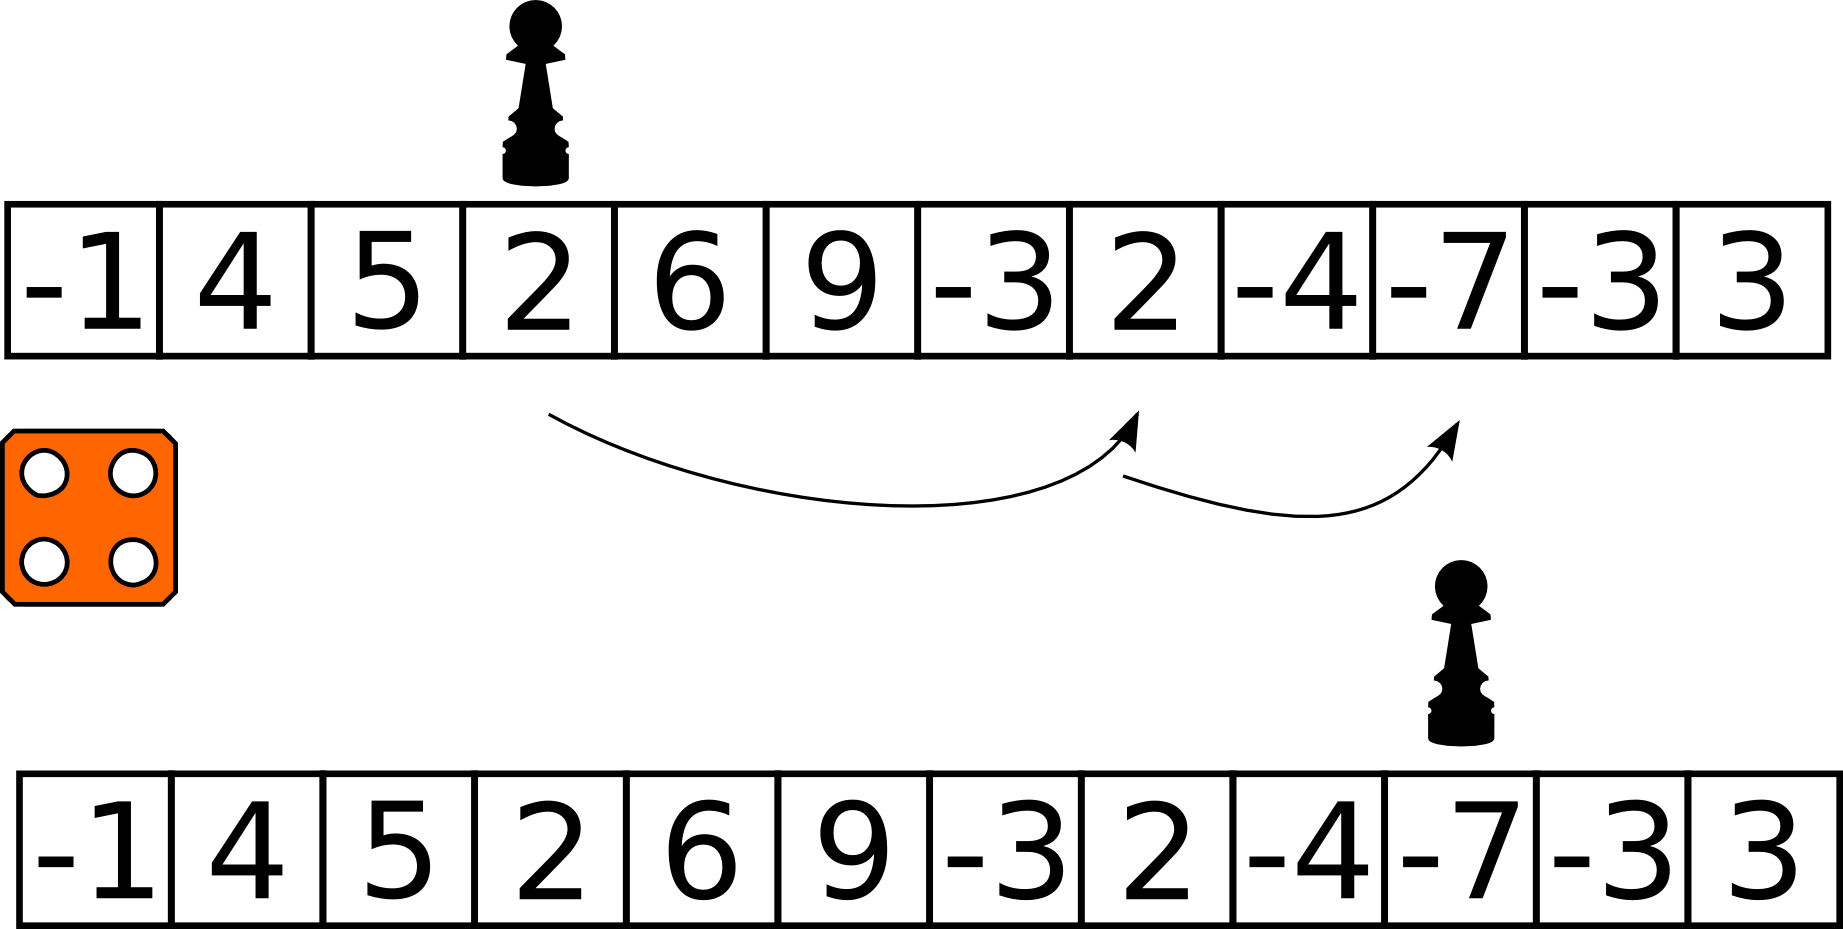
\includegraphics[width=280px]{images/snake-1}
			\end{center}
			
			Le premier joueur à atteindre ou dépasser la dernière case a gagné.
			Nous supposerons que cette dernière case est en position 42. Nous
			supposons également que la première et la dernière case n’ont ni
			échelle ni serpent (valeur nulle).
	
		\subsubsection*{Positions des joueurs}
		
			Les positions des joueurs seront mémorisées dans un tableau
			d’entiers.  Toutes les cases de ce tableau sont initialisées à 0. 
		
			Le plateau de jeu, un tableau d’entiers s’appellera \textbf{chemin}. 
		
			Le tableau d’entiers contenant la position courante des joueurs
			s’appellera \textbf{positionsJoueurs}. 
		
			S’il y a 4 joueurs, le tableau \textit{positionsJoueurs} contient 
			[2,5,1,7] alors~:
			\begin{itemize}
				\item le joueur 0 est en position 2 sur le chemin~;
				\item le joueur 1 est en position 5 sur le chemin~;
				\item le joueur 2 est en position 1 sur le chemin~;
				\item le joueur 3 est en position 7 sur le chemin~;
			\end{itemize}
				
		\subsubsection*{Le premier jour, initialiser le chemin}
		
			Écrivez un algorithme 
			\begin{java}
public static int[] créerChemin(int n)
			\end{java}
			
			Cet algorithme \textit{créerChemin} créera un tableau d’entiers dont
			les valeurs seront des valeurs aléatoires comprises strictement
			entre -10 et 10 (inclus). 
		
			Nous supposons que l’entier $n$ est un naturel strictement supérieur
			à 0.  Vous ne devez pas le vérifier. 
	
		\subsubsection*{Qui est en tête~?}
	
			Écrivez un algorithme 
	
			\begin{java}
public static int enPremièrePosition(int[] positionsJoueurs)
			\end{java}

			Cet algorithme retourne le numéro du joueur en tête de la course. 
			Il recherche donc le maximum dans le tableau passé en
			argument et retourne l’indice de ce maximum. 
	
		\subsubsection*{Jouer un tour de jeu}
	
			Cet algorithme permettra de jouer un tour de jeu pour un joueur
			donné. Jouer un tour de jeu consiste à le faire avancer ou reculer
			(c’est-à-dire changer sa position) du bon nombre de cases. 
	
			\begin{java}
public static void jouer(int[] chemin,
		int[] positionsJoueurs,
		int joueurCourant,
		int valeurDé)
			\end{java}
		
			Cet algorithme fait changer de position le joueur d’indice
			\textit{joueurCourant} de la valeur donnée par le dé
			(\textit{valeurDé}) en respectant les règles du jeu. 
		
			Cet algorithme met donc à jour le tableau \textit{positionsJoueurs}. 
		
			Comme le joueur ne peut se placer sur une case déjà occupée, il peut
			être utile d’écrire un module \texttt{estOccupé} précisant si la
			case est libre ou occupée.  
	
		\end{Exercice}


		\begin{Exercice}{Les algorithmes en maternelle}

		En maternelle, déjà, les enfants font des algorithmes 
		mais il s’agit d’une chose un peu différente.
		On leur propose un collier\footnote{%
			Par exemple, mais ça peut aussi être une chenille,
			un escargot, une simple suite de cases\dots
		}
		dessiné sur une feuille de papier 
		et ils doivent le colorier en répétant un
		\emph{motif} donné\footnote{%
			Ce qu’ils appellent un \emph{algorithme}.
		}, 
		une séquence précise de couleurs.
		
		Par exemple, on donne ce collier 
		 
		\perle{red}-\perle{red}-\perle{green}-\perle{white}-\perle{white}-\perle{white}-\perle{white}-\perle{white}-\perle{white}-\perle{white}\ 
		
		qui est précolorié avec deux perles rouges et une perle verte, c’est le
		motif\footnote{Pour cet exercice, le lecteur est content s'il a la
		version couleurs des notes.}.  
		
		Le résultat attendu est~:
		
		\perle{red}-\perle{red}-\perle{green}-\perle{red}-\perle{red}-\perle{green}-\perle{red}-\perle{red}-\perle{green}-\perle{red}.
		
		Comme on peut le constater sur cet exemple, un motif peut comporter
		plusieurs perles de la même couleur et, en fin de collier, il est
		possible qu’on ne puisse appliquer qu’une partie du motif.
		
		\textbf{Nous allons représenter chaque perle par un caractère
		indiquant sa couleur et un collier comme un tableau de caractères.
		Une perle non coloriée sera indiquée par un point (\Verb_'.'_).}
		
		Par exemple, le collier ci-dessus serait représenté ainsi~:
		
		\begin{center}
		\begin{tabular}{|*{10}{>{\centering\ttfamily\arraybackslash}m{6mm}|}}
		\hline
		'R' & 'R' & 'V' & '.' & '.' & '.' & '.' & '.' & '.' & '.' \\
		\hline
		\end{tabular}
		\end{center}
	
		\subsubsection*{Créer un collier}
		%-----------------------------------------
		
			Écrivez un algorithme \textbf{créerCollier}
			qui reçoit une taille et crée un collier de cette taille
			où toutes les perles sont non coloriées
			(rappel~: une perle non coloriée est représentée par un point).
			
			On suppose que la taille reçue est bien un entier non négatif.
	
		\subsubsection*{Créer un motif}
		%-----------------------------------------
		
			Écrivez un algorithme \textbf{créerMotif}
			qui reçoit un collier dont aucune perle n’est coloriée
			et qui colorie les premières en fonction des indications
			de l’utilisateur.
			
			Concrètement,
			l’utilisateur entre les couleurs des perles
			en spécifiant à chaque fois, après,
			s’il y a encore une perle à colorier.
			Dans notre exemple de la première page,
			l’utilisateur entrerait successivement~:
			'R', vrai, 'R', vrai, 'V', faux. 
			
			L’algorithme doit vérifier que l’utilisateur
			ne demande pas à colorier plus de perles
			qu’il n’y en a dans le collier.
	
		\subsubsection*{Taille du motif}
		%-----------------------------------------
	
			Écrivez un algorithme \textbf{tailleMotif}
			qui reçoit un collier dont seulement les premières perles sont coloriées
			(c’est le motif qu’il faudra suivre)
			et qui donne la taille de ce motif.
			Dans l’exemple de la première page, il faudra retourner la valeur 3.
			Votre algorithme doit générer une erreur si il n’y a pas de motif à suivre.
	
		\subsubsection*{Suivre un motif}
		%-----------------------------------------
		
			Écrivez un algorithme \textbf{colorier}
			qui reçoit un collier dont seulement les premières perles sont coloriées
			(c’est le motif qu’il faut suivre)
			et qui colorie le reste du collier en suivant ce motif.
			
		\subsubsection*{Vérifier un collier}
		%-----------------------------------------
		
			Écrivez un algorithme \textbf{vérifier}
			qui reçoit un collier complètement colorié
			et la taille du motif de départ et qui vérifie
			si le collier respecte ce motif.
		
		\subsubsection*{Trouver le motif}
		%-----------------------------------------
		
			Écrivez un algorithme \textbf{trouverMotif}
			qui reçoit un collier complètement colorié
			et qui détermine la taille du motif.
			C’est la plus petite séquence qui se répète.
			Comme cas extrème, ce pourrait être le collier tout entier.
		
			Aide~: vous avez déjà tout pour que cet exercice soit facile.


		\end{Exercice}

